\begin{figure}


	\centering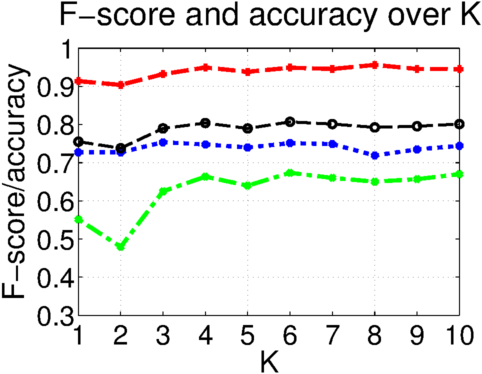
\includegraphics[width=0.3\textwidth]{scentroid2010FP.png}
	\centering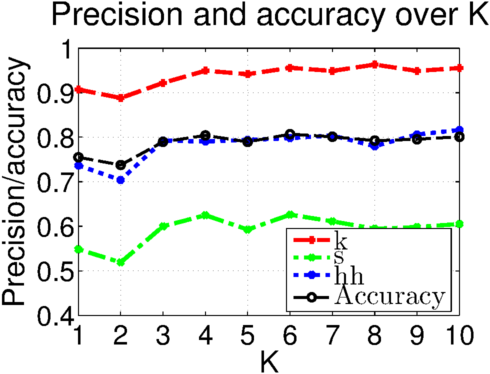
\includegraphics[width=0.3\textwidth]{scentroid2010_P.png}
	\centering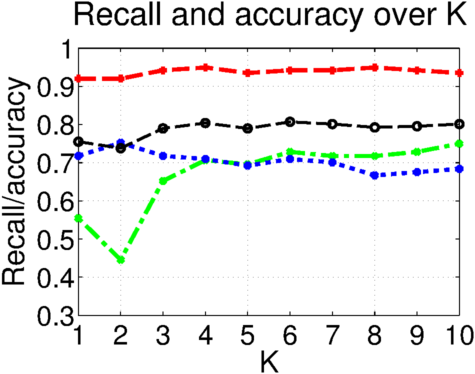
\includegraphics[width=0.3\textwidth]{scentroid2010_R.png}
	
	\caption{Plots over K for Spectral Centroid with 20ms windows and 10ms window skips}
\end{figure}
\begin{figure}


	\centering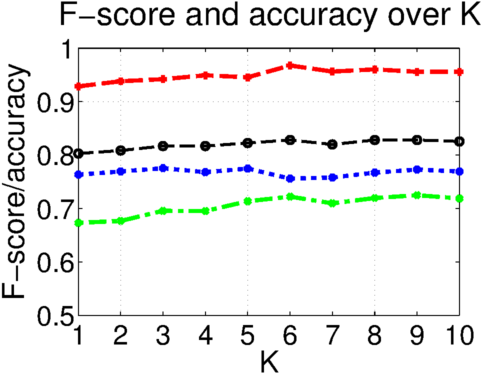
\includegraphics[width=0.3\textwidth]{scentroid105FP.png}
	\centering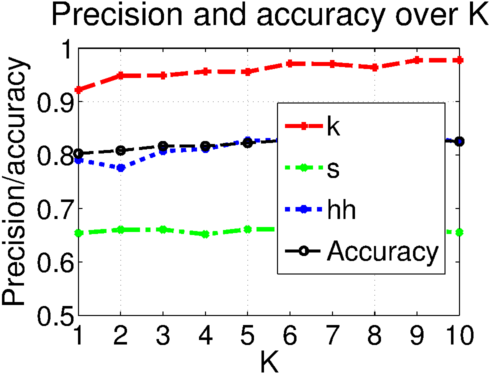
\includegraphics[width=0.3\textwidth]{scentroid105_P.png}
	\centering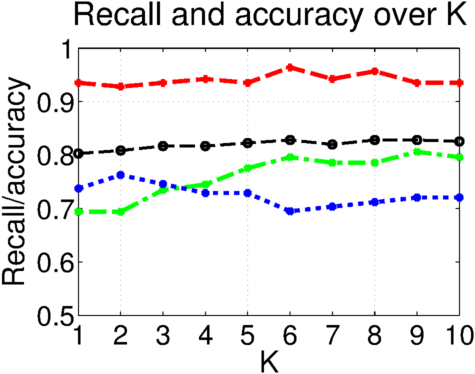
\includegraphics[width=0.3\textwidth]{scentroid105_R.png}
		
		\caption{Plots over K for Spectral Centroid with 10ms windows and 5ms window skips}
\end{figure}
\begin{figure}


	\centering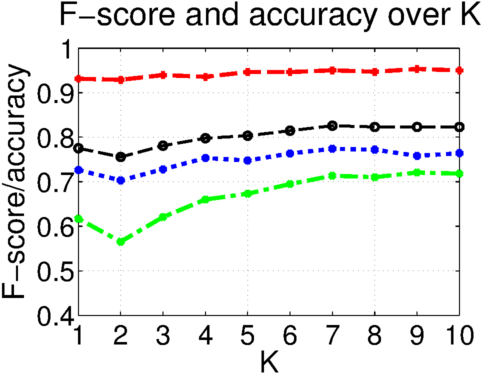
\includegraphics[width=0.3\textwidth]{scentroid52FP.png}
	\centering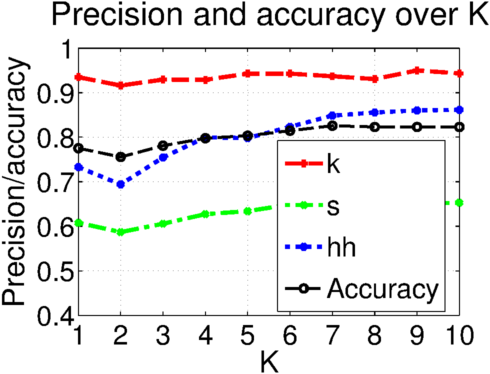
\includegraphics[width=0.3\textwidth]{scentroid52_P.png}
	\centering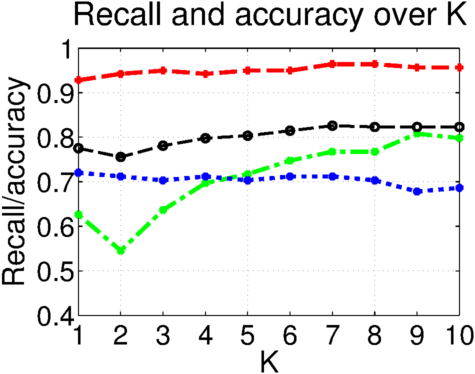
\includegraphics[width=0.3\textwidth]{scentroid52_R.png}
		
		\caption{Plots over K for Spectral Centroid with 5ms windows and 2ms window skips}
\end{figure}\clearpage

\begin{table}
\begin{subtable}[h]{0.45\textwidth}
\centering
\begin{tabular}{|c|c|c|c"c|}
\cline{2-5}
 \multicolumn{1}{c|}{} & \textbf{k}  & \textbf{s}  & \textbf{hh}  & Prec.\\ \hline
 \textbf{s} & \textcolor{red}{0.920} & 0.120 & 0.017 & 0.907\\ \hline
 \textbf{k} & 0.080 & \textcolor{red}{0.554} & 0.265 & 0.548\\ \hline
 \textbf{hh} & 0.080 & 0.326 & \textcolor{red}{0.718} & 0.737\\ \Xhline{2\arrayrulewidth}
 F & 0.914 & 0.551 & 0.727 & \textcolor{blue}{0.755}\\ \hline
\end{tabular}
\caption{$K=1$}
\end{subtable}
\hfill
\begin{subtable}[h]{0.45\textwidth}
\centering
\begin{tabular}{|c|c|c|c"c|}
\cline{2-5}
 \multicolumn{1}{c|}{} & \textbf{k}  & \textbf{s}  & \textbf{hh}  & Prec.\\ \hline
 \textbf{s} & \textcolor{red}{0.920} & 0.163 & 0.009 & 0.888\\ \hline
 \textbf{k} & 0.072 & \textcolor{red}{0.446} & 0.239 & 0.519\\ \hline
 \textbf{hh} & 0.072 & 0.391 & \textcolor{red}{0.752} & 0.704\\ \Xhline{2\arrayrulewidth}
 F & 0.904 & 0.480 & 0.727 & \textcolor{blue}{0.738}\\ \hline
\end{tabular}
\caption{$K=2$}
\end{subtable}
\hfill
\begin{subtable}[h]{0.45\textwidth}
\centering
\begin{tabular}{|c|c|c|c"c|}
\cline{2-5}
 \multicolumn{1}{c|}{} & \textbf{k}  & \textbf{s}  & \textbf{hh}  & Prec.\\ \hline
 \textbf{s} & \textcolor{red}{0.942} & 0.109 & 0.009 & 0.922\\ \hline
 \textbf{k} & 0.058 & \textcolor{red}{0.652} & 0.274 & 0.600\\ \hline
 \textbf{hh} & 0.058 & 0.239 & \textcolor{red}{0.718} & 0.792\\ \Xhline{2\arrayrulewidth}
 F & 0.932 & 0.625 & 0.753 & \textcolor{blue}{0.790}\\ \hline
\end{tabular}
\caption{$K=3$}
\end{subtable}
\hfill
\begin{subtable}[h]{0.45\textwidth}
\centering
\begin{tabular}{|c|c|c|c"c|}
\cline{2-5}
 \multicolumn{1}{c|}{} & \textbf{k}  & \textbf{s}  & \textbf{hh}  & Prec.\\ \hline
 \textbf{s} & \textcolor{red}{0.949} & 0.065 & 0.009 & 0.949\\ \hline
 \textbf{k} & 0.043 & \textcolor{red}{0.707} & 0.282 & 0.625\\ \hline
 \textbf{hh} & 0.043 & 0.228 & \textcolor{red}{0.709} & 0.790\\ \Xhline{2\arrayrulewidth}
 F & 0.949 & 0.663 & 0.748 & \textcolor{blue}{0.804}\\ \hline
\end{tabular}
\caption{$K=4$}
\end{subtable}
\hfill
\begin{subtable}[h]{0.45\textwidth}
\centering
\begin{tabular}{|c|c|c|c"c|}
\cline{2-5}
 \multicolumn{1}{c|}{} & \textbf{k}  & \textbf{s}  & \textbf{hh}  & Prec.\\ \hline
 \textbf{s} & \textcolor{red}{0.935} & 0.076 & 0.009 & 0.942\\ \hline
 \textbf{k} & 0.065 & \textcolor{red}{0.696} & 0.299 & 0.593\\ \hline
 \textbf{hh} & 0.065 & 0.228 & \textcolor{red}{0.692} & 0.794\\ \Xhline{2\arrayrulewidth}
 F & 0.938 & 0.640 & 0.740 & \textcolor{blue}{0.790}\\ \hline
\end{tabular}
\caption{$K=5$}
\end{subtable}
\hfill
\begin{subtable}[h]{0.45\textwidth}
\centering
\begin{tabular}{|c|c|c|c"c|}
\cline{2-5}
 \multicolumn{1}{c|}{} & \textbf{k}  & \textbf{s}  & \textbf{hh}  & Prec.\\ \hline
 \textbf{s} & \textcolor{red}{0.942} & 0.054 & 0.009 & 0.956\\ \hline
 \textbf{k} & 0.051 & \textcolor{red}{0.728} & 0.282 & 0.626\\ \hline
 \textbf{hh} & 0.051 & 0.217 & \textcolor{red}{0.709} & 0.798\\ \Xhline{2\arrayrulewidth}
 F & 0.949 & 0.673 & 0.751 & \textcolor{blue}{0.807}\\ \hline
\end{tabular}
\caption{$K=6$}
\end{subtable}
\hfill
\begin{subtable}[h]{0.45\textwidth}
\centering
\begin{tabular}{|c|c|c|c"c|}
\cline{2-5}
 \multicolumn{1}{c|}{} & \textbf{k}  & \textbf{s}  & \textbf{hh}  & Prec.\\ \hline
 \textbf{s} & \textcolor{red}{0.942} & 0.065 & 0.009 & 0.949\\ \hline
 \textbf{k} & 0.058 & \textcolor{red}{0.717} & 0.291 & 0.611\\ \hline
 \textbf{hh} & 0.058 & 0.217 & \textcolor{red}{0.701} & 0.804\\ \Xhline{2\arrayrulewidth}
 F & 0.945 & 0.660 & 0.749 & \textcolor{blue}{0.801}\\ \hline
\end{tabular}
\caption{$K=7$}
\end{subtable}
\hfill
\begin{subtable}[h]{0.45\textwidth}
\centering
\begin{tabular}{|c|c|c|c"c|}
\cline{2-5}
 \multicolumn{1}{c|}{} & \textbf{k}  & \textbf{s}  & \textbf{hh}  & Prec.\\ \hline
 \textbf{s} & \textcolor{red}{0.949} & 0.043 & 0.009 & 0.963\\ \hline
 \textbf{k} & 0.051 & \textcolor{red}{0.717} & 0.325 & 0.595\\ \hline
 \textbf{hh} & 0.051 & 0.239 & \textcolor{red}{0.667} & 0.780\\ \Xhline{2\arrayrulewidth}
 F & 0.956 & 0.650 & 0.719 & \textcolor{blue}{0.793}\\ \hline
\end{tabular}
\caption{$K=8$}
\end{subtable}
\hfill
\begin{subtable}[h]{0.45\textwidth}
\centering
\begin{tabular}{|c|c|c|c"c|}
\cline{2-5}
 \multicolumn{1}{c|}{} & \textbf{k}  & \textbf{s}  & \textbf{hh}  & Prec.\\ \hline
 \textbf{s} & \textcolor{red}{0.942} & 0.065 & 0.009 & 0.949\\ \hline
 \textbf{k} & 0.058 & \textcolor{red}{0.728} & 0.316 & 0.598\\ \hline
 \textbf{hh} & 0.058 & 0.207 & \textcolor{red}{0.675} & 0.806\\ \Xhline{2\arrayrulewidth}
 F & 0.945 & 0.657 & 0.735 & \textcolor{blue}{0.795}\\ \hline
\end{tabular}
\caption{$K=9$}
\end{subtable}
\hfill
\begin{subtable}[h]{0.45\textwidth}
\centering
\begin{tabular}{|c|c|c|c"c|}
\cline{2-5}
 \multicolumn{1}{c|}{} & \textbf{k}  & \textbf{s}  & \textbf{hh}  & Prec.\\ \hline
 \textbf{s} & \textcolor{red}{0.935} & 0.054 & 0.009 & 0.956\\ \hline
 \textbf{k} & 0.065 & \textcolor{red}{0.750} & 0.308 & 0.605\\ \hline
 \textbf{hh} & 0.065 & 0.196 & \textcolor{red}{0.684} & 0.816\\ \Xhline{2\arrayrulewidth}
 F & 0.945 & 0.670 & 0.744 & \textcolor{blue}{0.801}\\ \hline
\end{tabular}
\caption{$K=10$}
\end{subtable}
\hfill

\label{tlscentroid2010}

\caption{tcscentroid2010}

\end{table}

\newcolumntype{"}{@{\hskip\tabcolsep\vrule width 1pt\hskip\tabcolsep}}
\begin{table}

\begin{subtable}[h]{0.45\textwidth}
\centering
\scalebox{0.8}{
\begin{tabular}{|c|c|c|c|}\hline
 $K_1$ & $K_2$ & $X^2$ & p\\ \hline
 1 & 2 & 54.000 & 0.00643\\ \hline 
 1 & 3 & 63.000 & 0.00539\\ \hline 
 1 & 4 & 54.000 & 0.00225\\ \hline 
 1 & 5 & 63.000 & 0.00539\\ \hline 
 1 & 6 & 54.000 & 0.00643\\ \hline 
 1 & 7 & 63.000 & 0.00539\\ \hline 
 1 & 8 & 63.000 & 0.00539\\ \hline 
 1 & 9 & 63.000 & 0.00539\\ \hline 
 1 & 10 & 63.000 & 0.00539\\ \hline 
 2 & 3 & 63.000 & 0.00539\\ \hline 
 2 & 4 & 54.000 & 0.00225\\ \hline 
 2 & 5 & 63.000 & 0.00539\\ \hline 
 2 & 6 & 63.000 & 0.00192\\ \hline 
 2 & 7 & 63.000 & 0.00539\\ \hline 
 2 & 8 & 63.000 & 0.00539\\ \hline 
 2 & 9 & 63.000 & 0.00539\\ \hline 
 2 & 10 & 63.000 & 0.00539\\ \hline 
 3 & 4 & 54.000 & 0.00569\\ \hline 
 3 & 5 & 72.000 & 0.00512\\ \hline 
 3 & 6 & 63.000 & 0.00539\\ \hline 
 3 & 7 & 72.000 & 0.00512\\ \hline 
 3 & 8 & 72.000 & 0.00512\\ \hline 
 3 & 9 & 72.000 & 0.00512\\ \hline 
 3 & 10 & 72.000 & 0.00512\\ \hline 
 4 & 5 & 54.000 & 0.00569\\ \hline 
 4 & 6 & 54.000 & 0.00225\\ \hline 
 4 & 7 & 54.000 & 0.00569\\ \hline 
 4 & 8 & 54.000 & 0.00569\\ \hline 
 4 & 9 & 54.000 & 0.00569\\ \hline 
 4 & 10 & 54.000 & 0.00569\\ \hline 
 5 & 6 & 63.000 & 0.00539\\ \hline 
 5 & 7 & 72.000 & 0.00512\\ \hline 
 5 & 8 & 72.000 & 0.00512\\ \hline 
 5 & 9 & 72.000 & 0.00512\\ \hline 
 5 & 10 & 72.000 & 0.00512\\ \hline 
 6 & 7 & 63.000 & 0.00539\\ \hline 
 6 & 8 & 63.000 & 0.00539\\ \hline 
 6 & 9 & 63.000 & 0.00539\\ \hline 
 6 & 10 & 63.000 & 0.00539\\ \hline 
 7 & 8 & 72.000 & 0.00512\\ \hline 
 7 & 9 & 72.000 & 0.00512\\ \hline 
 7 & 10 & 72.000 & 0.00512\\ \hline 
 8 & 9 & 72.000 & 0.00512\\ \hline 
 8 & 10 & 72.000 & 0.00512\\ \hline 
 9 & 10 & 72.000 & 0.00512\\ \hline 

\end{tabular}
}\label{xlscentroid2010}
\caption{xcscentroid2010}
\end{subtable}

\begin{subtable}[h]{0.45\textwidth}
\centering
\begin{tabular}{|c|c|c|}
\hline
Class & Amount & Percent\\ \hline
k & 461 & 32.93\\ \hline
undefined & 125 & 8.93\\ \hline
s & 307 & 21.93\\ \hline
\end{tabular}
\caption{Entire dataset after stripping short sounds}
\end{subtable}
\hfill
\begin{subtable}[h]{0.45\textwidth}
\centering
\begin{tabular}{|c|c|c|}
\hline
Class & Amount & Percent\\ \hline
k & 322 & 39.80\\ \hline
s & 214 & 26.45\\ \hline
hh & 273 & 33.75\\ \hline
\end{tabular}
\caption{Training dataset}
\end{subtable}
\hfill
\begin{subtable}[h]{0.45\textwidth}
\centering
\begin{tabular}{|c|c|c|}
\hline
Class & Amount & Percent\\ \hline
k & 138 & 39.77\\ \hline
s & 92 & 26.51\\ \hline
hh & 117 & 33.72\\ \hline
\end{tabular}
\caption{Testing dataset}
\end{subtable}
\hfill

\label{dlscentroid2010}

\caption{dcscentroid2010}

\end{table}

\begin{table}
\begin{subtable}[h]{0.45\textwidth}
\centering
\begin{tabular}{|c|c|c|c"c|}
\cline{2-5}
 \multicolumn{1}{c|}{} & \textbf{k}  & \textbf{s}  & \textbf{hh}  & Prec.\\ \hline
 \textbf{s} & \textcolor{red}{0.935} & 0.082 & 0.025 & 0.922\\ \hline
 \textbf{k} & 0.058 & \textcolor{red}{0.694} & 0.237 & 0.654\\ \hline
 \textbf{hh} & 0.058 & 0.224 & \textcolor{red}{0.737} & 0.791\\ \Xhline{2\arrayrulewidth}
 F & 0.929 & 0.673 & 0.763 & \textcolor{blue}{0.803}\\ \hline
\end{tabular}
\caption{$K=1$}
\end{subtable}
\hfill
\begin{subtable}[h]{0.45\textwidth}
\centering
\begin{tabular}{|c|c|c|c"c|}
\cline{2-5}
 \multicolumn{1}{c|}{} & \textbf{k}  & \textbf{s}  & \textbf{hh}  & Prec.\\ \hline
 \textbf{s} & \textcolor{red}{0.928} & 0.041 & 0.025 & 0.949\\ \hline
 \textbf{k} & 0.072 & \textcolor{red}{0.694} & 0.212 & 0.660\\ \hline
 \textbf{hh} & 0.072 & 0.265 & \textcolor{red}{0.763} & 0.776\\ \Xhline{2\arrayrulewidth}
 F & 0.938 & 0.677 & 0.769 & \textcolor{blue}{0.808}\\ \hline
\end{tabular}
\caption{$K=2$}
\end{subtable}
\hfill
\begin{subtable}[h]{0.45\textwidth}
\centering
\begin{tabular}{|c|c|c|c"c|}
\cline{2-5}
 \multicolumn{1}{c|}{} & \textbf{k}  & \textbf{s}  & \textbf{hh}  & Prec.\\ \hline
 \textbf{s} & \textcolor{red}{0.935} & 0.051 & 0.017 & 0.949\\ \hline
 \textbf{k} & 0.065 & \textcolor{red}{0.735} & 0.237 & 0.661\\ \hline
 \textbf{hh} & 0.065 & 0.214 & \textcolor{red}{0.746} & 0.807\\ \Xhline{2\arrayrulewidth}
 F & 0.942 & 0.696 & 0.775 & \textcolor{blue}{0.817}\\ \hline
\end{tabular}
\caption{$K=3$}
\end{subtable}
\hfill
\begin{subtable}[h]{0.45\textwidth}
\centering
\begin{tabular}{|c|c|c|c"c|}
\cline{2-5}
 \multicolumn{1}{c|}{} & \textbf{k}  & \textbf{s}  & \textbf{hh}  & Prec.\\ \hline
 \textbf{s} & \textcolor{red}{0.942} & 0.051 & 0.008 & 0.956\\ \hline
 \textbf{k} & 0.058 & \textcolor{red}{0.745} & 0.263 & 0.652\\ \hline
 \textbf{hh} & 0.058 & 0.204 & \textcolor{red}{0.729} & 0.811\\ \Xhline{2\arrayrulewidth}
 F & 0.949 & 0.695 & 0.768 & \textcolor{blue}{0.817}\\ \hline
\end{tabular}
\caption{$K=4$}
\end{subtable}
\hfill
\begin{subtable}[h]{0.45\textwidth}
\centering
\begin{tabular}{|c|c|c|c"c|}
\cline{2-5}
 \multicolumn{1}{c|}{} & \textbf{k}  & \textbf{s}  & \textbf{hh}  & Prec.\\ \hline
 \textbf{s} & \textcolor{red}{0.935} & 0.041 & 0.017 & 0.956\\ \hline
 \textbf{k} & 0.065 & \textcolor{red}{0.776} & 0.254 & 0.661\\ \hline
 \textbf{hh} & 0.065 & 0.184 & \textcolor{red}{0.729} & 0.827\\ \Xhline{2\arrayrulewidth}
 F & 0.945 & 0.714 & 0.775 & \textcolor{blue}{0.823}\\ \hline
\end{tabular}
\caption{$K=5$}
\end{subtable}
\hfill
\begin{subtable}[h]{0.45\textwidth}
\centering
\begin{tabular}{|c|c|c|c"c|}
\cline{2-5}
 \multicolumn{1}{c|}{} & \textbf{k}  & \textbf{s}  & \textbf{hh}  & Prec.\\ \hline
 \textbf{s} & \textcolor{red}{0.964} & 0.031 & 0.008 & 0.971\\ \hline
 \textbf{k} & 0.036 & \textcolor{red}{0.796} & 0.297 & 0.661\\ \hline
 \textbf{hh} & 0.036 & 0.173 & \textcolor{red}{0.695} & 0.828\\ \Xhline{2\arrayrulewidth}
 F & 0.968 & 0.722 & 0.756 & \textcolor{blue}{0.828}\\ \hline
\end{tabular}
\caption{$K=6$}
\end{subtable}
\hfill
\begin{subtable}[h]{0.45\textwidth}
\centering
\begin{tabular}{|c|c|c|c"c|}
\cline{2-5}
 \multicolumn{1}{c|}{} & \textbf{k}  & \textbf{s}  & \textbf{hh}  & Prec.\\ \hline
 \textbf{s} & \textcolor{red}{0.942} & 0.031 & 0.008 & 0.970\\ \hline
 \textbf{k} & 0.058 & \textcolor{red}{0.786} & 0.288 & 0.647\\ \hline
 \textbf{hh} & 0.058 & 0.184 & \textcolor{red}{0.703} & 0.822\\ \Xhline{2\arrayrulewidth}
 F & 0.956 & 0.710 & 0.758 & \textcolor{blue}{0.820}\\ \hline
\end{tabular}
\caption{$K=7$}
\end{subtable}
\hfill
\begin{subtable}[h]{0.45\textwidth}
\centering
\begin{tabular}{|c|c|c|c"c|}
\cline{2-5}
 \multicolumn{1}{c|}{} & \textbf{k}  & \textbf{s}  & \textbf{hh}  & Prec.\\ \hline
 \textbf{s} & \textcolor{red}{0.957} & 0.041 & 0.008 & 0.964\\ \hline
 \textbf{k} & 0.043 & \textcolor{red}{0.786} & 0.280 & 0.664\\ \hline
 \textbf{hh} & 0.043 & 0.173 & \textcolor{red}{0.712} & 0.832\\ \Xhline{2\arrayrulewidth}
 F & 0.960 & 0.720 & 0.767 & \textcolor{blue}{0.828}\\ \hline
\end{tabular}
\caption{$K=8$}
\end{subtable}
\hfill
\begin{subtable}[h]{0.45\textwidth}
\centering
\begin{tabular}{|c|c|c|c"c|}
\cline{2-5}
 \multicolumn{1}{c|}{} & \textbf{k}  & \textbf{s}  & \textbf{hh}  & Prec.\\ \hline
 \textbf{s} & \textcolor{red}{0.935} & 0.020 & 0.008 & 0.977\\ \hline
 \textbf{k} & 0.065 & \textcolor{red}{0.806} & 0.271 & 0.658\\ \hline
 \textbf{hh} & 0.065 & 0.173 & \textcolor{red}{0.720} & 0.833\\ \Xhline{2\arrayrulewidth}
 F & 0.956 & 0.725 & 0.773 & \textcolor{blue}{0.828}\\ \hline
\end{tabular}
\caption{$K=9$}
\end{subtable}
\hfill
\begin{subtable}[h]{0.45\textwidth}
\centering
\begin{tabular}{|c|c|c|c"c|}
\cline{2-5}
 \multicolumn{1}{c|}{} & \textbf{k}  & \textbf{s}  & \textbf{hh}  & Prec.\\ \hline
 \textbf{s} & \textcolor{red}{0.935} & 0.020 & 0.008 & 0.977\\ \hline
 \textbf{k} & 0.065 & \textcolor{red}{0.796} & 0.271 & 0.655\\ \hline
 \textbf{hh} & 0.065 & 0.184 & \textcolor{red}{0.720} & 0.825\\ \Xhline{2\arrayrulewidth}
 F & 0.956 & 0.719 & 0.769 & \textcolor{blue}{0.825}\\ \hline
\end{tabular}
\caption{$K=10$}
\end{subtable}
\hfill

\label{tlscentroid105}

\caption{tcscentroid105}

\end{table}

\begin{table}

\begin{subtable}[h]{0.45\textwidth}
\centering
\scalebox{0.8}{
\begin{tabular}{|c|c|c|c|}\hline
 $K_1$ & $K_2$ & $X^2$ & p\\ \hline
 1 & 2 & 63.000 & 0.00539\\ \hline 
 1 & 3 & 63.000 & 0.00539\\ \hline 
 1 & 4 & 63.000 & 0.00539\\ \hline 
 1 & 5 & 63.000 & 0.00539\\ \hline 
 1 & 6 & 63.000 & 0.00539\\ \hline 
 1 & 7 & 63.000 & 0.00539\\ \hline 
 1 & 8 & 63.000 & 0.00539\\ \hline 
 1 & 9 & 63.000 & 0.00539\\ \hline 
 1 & 10 & 63.000 & 0.00539\\ \hline 
 2 & 3 & 72.000 & 0.00512\\ \hline 
 2 & 4 & 72.000 & 0.00512\\ \hline 
 2 & 5 & 72.000 & 0.00512\\ \hline 
 2 & 6 & 72.000 & 0.00512\\ \hline 
 2 & 7 & 72.000 & 0.00512\\ \hline 
 2 & 8 & 72.000 & 0.00512\\ \hline 
 2 & 9 & 72.000 & 0.00512\\ \hline 
 2 & 10 & 72.000 & 0.00512\\ \hline 
 3 & 4 & 72.000 & 0.00512\\ \hline 
 3 & 5 & 72.000 & 0.00512\\ \hline 
 3 & 6 & 72.000 & 0.00512\\ \hline 
 3 & 7 & 72.000 & 0.00512\\ \hline 
 3 & 8 & 72.000 & 0.00512\\ \hline 
 3 & 9 & 72.000 & 0.00512\\ \hline 
 3 & 10 & 72.000 & 0.00512\\ \hline 
 4 & 5 & 72.000 & 0.00512\\ \hline 
 4 & 6 & 72.000 & 0.00512\\ \hline 
 4 & 7 & 72.000 & 0.00512\\ \hline 
 4 & 8 & 72.000 & 0.00512\\ \hline 
 4 & 9 & 72.000 & 0.00512\\ \hline 
 4 & 10 & 72.000 & 0.00512\\ \hline 
 5 & 6 & 72.000 & 0.00512\\ \hline 
 5 & 7 & 72.000 & 0.00512\\ \hline 
 5 & 8 & 72.000 & 0.00512\\ \hline 
 5 & 9 & 72.000 & 0.00512\\ \hline 
 5 & 10 & 72.000 & 0.00512\\ \hline 
 6 & 7 & 72.000 & 0.00512\\ \hline 
 6 & 8 & 72.000 & 0.00512\\ \hline 
 6 & 9 & 72.000 & 0.00512\\ \hline 
 6 & 10 & 72.000 & 0.00512\\ \hline 
 7 & 8 & 72.000 & 0.00512\\ \hline 
 7 & 9 & 72.000 & 0.00512\\ \hline 
 7 & 10 & 72.000 & 0.00512\\ \hline 
 8 & 9 & 72.000 & 0.00512\\ \hline 
 8 & 10 & 72.000 & 0.00512\\ \hline 
 9 & 10 & 72.000 & 0.00512\\ \hline 

\end{tabular}
}\label{xlscentroid105}
\caption{xcscentroid105}
\end{subtable}

\begin{subtable}[h]{0.45\textwidth}
\centering
\begin{tabular}{|c|c|c|}
\hline
Class & Amount & Percent\\ \hline
noise & 138 & 9.47\\ \hline
k & 466 & 31.98\\ \hline
undefined & 130 & 8.92\\ \hline
\end{tabular}
\caption{Entire dataset after stripping short sounds}
\end{subtable}
\hfill
\begin{subtable}[h]{0.45\textwidth}
\centering
\begin{tabular}{|c|c|c|}
\hline
Class & Amount & Percent\\ \hline
k & 326 & 39.23\\ \hline
s & 229 & 27.56\\ \hline
hh & 276 & 33.21\\ \hline
\end{tabular}
\caption{Training dataset}
\end{subtable}
\hfill
\begin{subtable}[h]{0.45\textwidth}
\centering
\begin{tabular}{|c|c|c|}
\hline
Class & Amount & Percent\\ \hline
k & 139 & 39.15\\ \hline
s & 98 & 27.61\\ \hline
hh & 118 & 33.24\\ \hline
\end{tabular}
\caption{Testing dataset}
\end{subtable}
\hfill

\label{dlscentroid105}

\caption{dcscentroid105}

\end{table}\clearpage

\begin{table}
\begin{subtable}[h]{0.45\textwidth}
\centering
\begin{tabular}{|c|c|c|c"c|}
\cline{2-5}
 \multicolumn{1}{c|}{} & \textbf{k}  & \textbf{s}  & \textbf{hh}  & Prec.\\ \hline
 \textbf{s} & \textcolor{red}{0.928} & 0.071 & 0.017 & 0.935\\ \hline
 \textbf{k} & 0.065 & \textcolor{red}{0.626} & 0.263 & 0.608\\ \hline
 \textbf{hh} & 0.065 & 0.303 & \textcolor{red}{0.720} & 0.733\\ \Xhline{2\arrayrulewidth}
 F & 0.931 & 0.617 & 0.726 & \textcolor{blue}{0.775}\\ \hline
\end{tabular}
\caption{$K=1$}
\end{subtable}
\hfill
\begin{subtable}[h]{0.45\textwidth}
\centering
\begin{tabular}{|c|c|c|c"c|}
\cline{2-5}
 \multicolumn{1}{c|}{} & \textbf{k}  & \textbf{s}  & \textbf{hh}  & Prec.\\ \hline
 \textbf{s} & \textcolor{red}{0.942} & 0.091 & 0.025 & 0.916\\ \hline
 \textbf{k} & 0.050 & \textcolor{red}{0.545} & 0.263 & 0.587\\ \hline
 \textbf{hh} & 0.050 & 0.364 & \textcolor{red}{0.712} & 0.694\\ \Xhline{2\arrayrulewidth}
 F & 0.929 & 0.565 & 0.703 & \textcolor{blue}{0.756}\\ \hline
\end{tabular}
\caption{$K=2$}
\end{subtable}
\hfill
\begin{subtable}[h]{0.45\textwidth}
\centering
\begin{tabular}{|c|c|c|c"c|}
\cline{2-5}
 \multicolumn{1}{c|}{} & \textbf{k}  & \textbf{s}  & \textbf{hh}  & Prec.\\ \hline
 \textbf{s} & \textcolor{red}{0.950} & 0.091 & 0.008 & 0.930\\ \hline
 \textbf{k} & 0.050 & \textcolor{red}{0.636} & 0.288 & 0.606\\ \hline
 \textbf{hh} & 0.050 & 0.273 & \textcolor{red}{0.703} & 0.755\\ \Xhline{2\arrayrulewidth}
 F & 0.940 & 0.621 & 0.728 & \textcolor{blue}{0.781}\\ \hline
\end{tabular}
\caption{$K=3$}
\end{subtable}
\hfill
\begin{subtable}[h]{0.45\textwidth}
\centering
\begin{tabular}{|c|c|c|c"c|}
\cline{2-5}
 \multicolumn{1}{c|}{} & \textbf{k}  & \textbf{s}  & \textbf{hh}  & Prec.\\ \hline
 \textbf{s} & \textcolor{red}{0.942} & 0.091 & 0.008 & 0.929\\ \hline
 \textbf{k} & 0.058 & \textcolor{red}{0.697} & 0.280 & 0.627\\ \hline
 \textbf{hh} & 0.058 & 0.212 & \textcolor{red}{0.712} & 0.800\\ \Xhline{2\arrayrulewidth}
 F & 0.936 & 0.660 & 0.753 & \textcolor{blue}{0.798}\\ \hline
\end{tabular}
\caption{$K=4$}
\end{subtable}
\hfill
\begin{subtable}[h]{0.45\textwidth}
\centering
\begin{tabular}{|c|c|c|c"c|}
\cline{2-5}
 \multicolumn{1}{c|}{} & \textbf{k}  & \textbf{s}  & \textbf{hh}  & Prec.\\ \hline
 \textbf{s} & \textcolor{red}{0.950} & 0.071 & 0.008 & 0.943\\ \hline
 \textbf{k} & 0.050 & \textcolor{red}{0.717} & 0.288 & 0.634\\ \hline
 \textbf{hh} & 0.050 & 0.212 & \textcolor{red}{0.703} & 0.798\\ \Xhline{2\arrayrulewidth}
 F & 0.946 & 0.673 & 0.748 & \textcolor{blue}{0.803}\\ \hline
\end{tabular}
\caption{$K=5$}
\end{subtable}
\hfill
\begin{subtable}[h]{0.45\textwidth}
\centering
\begin{tabular}{|c|c|c|c"c|}
\cline{2-5}
 \multicolumn{1}{c|}{} & \textbf{k}  & \textbf{s}  & \textbf{hh}  & Prec.\\ \hline
 \textbf{s} & \textcolor{red}{0.950} & 0.071 & 0.008 & 0.943\\ \hline
 \textbf{k} & 0.050 & \textcolor{red}{0.747} & 0.280 & 0.649\\ \hline
 \textbf{hh} & 0.050 & 0.182 & \textcolor{red}{0.712} & 0.824\\ \Xhline{2\arrayrulewidth}
 F & 0.946 & 0.695 & 0.764 & \textcolor{blue}{0.815}\\ \hline
\end{tabular}
\caption{$K=6$}
\end{subtable}
\hfill
\begin{subtable}[h]{0.45\textwidth}
\centering
\begin{tabular}{|c|c|c|c"c|}
\cline{2-5}
 \multicolumn{1}{c|}{} & \textbf{k}  & \textbf{s}  & \textbf{hh}  & Prec.\\ \hline
 \textbf{s} & \textcolor{red}{0.964} & 0.081 & 0.008 & 0.937\\ \hline
 \textbf{k} & 0.036 & \textcolor{red}{0.768} & 0.280 & 0.667\\ \hline
 \textbf{hh} & 0.036 & 0.152 & \textcolor{red}{0.712} & 0.848\\ \Xhline{2\arrayrulewidth}
 F & 0.950 & 0.714 & 0.774 & \textcolor{blue}{0.826}\\ \hline
\end{tabular}
\caption{$K=7$}
\end{subtable}
\hfill
\begin{subtable}[h]{0.45\textwidth}
\centering
\begin{tabular}{|c|c|c|c"c|}
\cline{2-5}
 \multicolumn{1}{c|}{} & \textbf{k}  & \textbf{s}  & \textbf{hh}  & Prec.\\ \hline
 \textbf{s} & \textcolor{red}{0.964} & 0.091 & 0.008 & 0.931\\ \hline
 \textbf{k} & 0.036 & \textcolor{red}{0.768} & 0.288 & 0.661\\ \hline
 \textbf{hh} & 0.036 & 0.141 & \textcolor{red}{0.703} & 0.856\\ \Xhline{2\arrayrulewidth}
 F & 0.947 & 0.710 & 0.772 & \textcolor{blue}{0.823}\\ \hline
\end{tabular}
\caption{$K=8$}
\end{subtable}
\hfill
\begin{subtable}[h]{0.45\textwidth}
\centering
\begin{tabular}{|c|c|c|c"c|}
\cline{2-5}
 \multicolumn{1}{c|}{} & \textbf{k}  & \textbf{s}  & \textbf{hh}  & Prec.\\ \hline
 \textbf{s} & \textcolor{red}{0.957} & 0.061 & 0.008 & 0.950\\ \hline
 \textbf{k} & 0.043 & \textcolor{red}{0.808} & 0.314 & 0.650\\ \hline
 \textbf{hh} & 0.043 & 0.131 & \textcolor{red}{0.678} & 0.860\\ \Xhline{2\arrayrulewidth}
 F & 0.953 & 0.721 & 0.758 & \textcolor{blue}{0.823}\\ \hline
\end{tabular}
\caption{$K=9$}
\end{subtable}
\hfill
\begin{subtable}[h]{0.45\textwidth}
\centering
\begin{tabular}{|c|c|c|c"c|}
\cline{2-5}
 \multicolumn{1}{c|}{} & \textbf{k}  & \textbf{s}  & \textbf{hh}  & Prec.\\ \hline
 \textbf{s} & \textcolor{red}{0.957} & 0.071 & 0.008 & 0.943\\ \hline
 \textbf{k} & 0.043 & \textcolor{red}{0.798} & 0.305 & 0.653\\ \hline
 \textbf{hh} & 0.043 & 0.131 & \textcolor{red}{0.686} & 0.862\\ \Xhline{2\arrayrulewidth}
 F & 0.950 & 0.718 & 0.764 & \textcolor{blue}{0.823}\\ \hline
\end{tabular}
\caption{$K=10$}
\end{subtable}
\hfill

\label{tlscentroid52}

\caption{tcscentroid52}

\end{table}\clearpage

\begin{table}

\begin{subtable}[h]{0.45\textwidth}
\centering
\scalebox{0.8}{
\begin{tabular}{|c|c|c|c|}\hline
 $K_1$ & $K_2$ & $X^2$ & p\\ \hline
 1 & 2 & 72.000 & 0.00512\\ \hline 
 1 & 3 & 72.000 & 0.00512\\ \hline 
 1 & 4 & 72.000 & 0.00512\\ \hline 
 1 & 5 & 63.000 & 0.00539\\ \hline 
 1 & 6 & 63.000 & 0.00539\\ \hline 
 1 & 7 & 72.000 & 0.00512\\ \hline 
 1 & 8 & 72.000 & 0.00512\\ \hline 
 1 & 9 & 54.000 & 0.00569\\ \hline 
 1 & 10 & 72.000 & 0.00512\\ \hline 
 2 & 3 & 72.000 & 0.00512\\ \hline 
 2 & 4 & 72.000 & 0.00512\\ \hline 
 2 & 5 & 63.000 & 0.00539\\ \hline 
 2 & 6 & 63.000 & 0.00539\\ \hline 
 2 & 7 & 72.000 & 0.00512\\ \hline 
 2 & 8 & 72.000 & 0.00512\\ \hline 
 2 & 9 & 54.000 & 0.00569\\ \hline 
 2 & 10 & 72.000 & 0.00512\\ \hline 
 3 & 4 & 72.000 & 0.00512\\ \hline 
 3 & 5 & 63.000 & 0.00539\\ \hline 
 3 & 6 & 63.000 & 0.00539\\ \hline 
 3 & 7 & 72.000 & 0.00512\\ \hline 
 3 & 8 & 72.000 & 0.00512\\ \hline 
 3 & 9 & 54.000 & 0.00569\\ \hline 
 3 & 10 & 72.000 & 0.00512\\ \hline 
 4 & 5 & 63.000 & 0.00539\\ \hline 
 4 & 6 & 63.000 & 0.00539\\ \hline 
 4 & 7 & 72.000 & 0.00512\\ \hline 
 4 & 8 & 72.000 & 0.00512\\ \hline 
 4 & 9 & 54.000 & 0.00569\\ \hline 
 4 & 10 & 72.000 & 0.00512\\ \hline 
 5 & 6 & 63.000 & 0.00192\\ \hline 
 5 & 7 & 63.000 & 0.00539\\ \hline 
 5 & 8 & 63.000 & 0.00539\\ \hline 
 5 & 9 & 54.000 & 0.00225\\ \hline 
 5 & 10 & 63.000 & 0.00539\\ \hline 
 6 & 7 & 63.000 & 0.00539\\ \hline 
 6 & 8 & 63.000 & 0.00539\\ \hline 
 6 & 9 & 54.000 & 0.00225\\ \hline 
 6 & 10 & 63.000 & 0.00539\\ \hline 
 7 & 8 & 72.000 & 0.00512\\ \hline 
 7 & 9 & 54.000 & 0.00569\\ \hline 
 7 & 10 & 72.000 & 0.00512\\ \hline 
 8 & 9 & 54.000 & 0.00569\\ \hline 
 8 & 10 & 72.000 & 0.00512\\ \hline 
 9 & 10 & 54.000 & 0.00569\\ \hline 

\end{tabular}
}\label{xlscentroid52}
\caption{xcscentroid52}
\end{subtable}

\begin{subtable}[h]{0.45\textwidth}
\centering
\begin{tabular}{|c|c|c|}
\hline
Class & Amount & Percent\\ \hline
noise & 148 & 10.07\\ \hline
k & 466 & 31.70\\ \hline
undefined & 130 & 8.84\\ \hline
\end{tabular}
\caption{Entire dataset after stripping short sounds}
\end{subtable}
\hfill
\begin{subtable}[h]{0.45\textwidth}
\centering
\begin{tabular}{|c|c|c|}
\hline
Class & Amount & Percent\\ \hline
k & 326 & 39.14\\ \hline
s & 231 & 27.73\\ \hline
hh & 276 & 33.13\\ \hline
\end{tabular}
\caption{Training dataset}
\end{subtable}
\hfill
\begin{subtable}[h]{0.45\textwidth}
\centering
\begin{tabular}{|c|c|c|}
\hline
Class & Amount & Percent\\ \hline
k & 139 & 39.04\\ \hline
s & 99 & 27.81\\ \hline
hh & 118 & 33.15\\ \hline
\end{tabular}
\caption{Testing dataset}
\end{subtable}
\hfill

\label{dlscentroid52}

\caption{dcscentroid52}

\end{table}\clearpage
